\documentclass[border=4pt]{standalone}
\usepackage{fontspec}
\usepackage{amsmath}
\usepackage{unicode-math}
\setmainfont{Latin Modern Roman}
\setmathfont{Latin Modern Math}
\usepackage{pgfplots}
\usepackage{pgfplotstable}
\pgfplotsset{compat=1.18}
\usepackage{tkz-euclide}
\usetikzlibrary{arrows.meta,calc,angles,quotes,patterns,3d,backgrounds}
\definecolor{ink}{HTML}{123428}
\definecolor{asy}{HTML}{475569}
\definecolor{mint}{HTML}{86e0bd}
\tikzset{asym/.style={asy, line width=0.9pt, dash pattern=on 5pt off 3.5pt},
         guide/.style={gray!70, line width=0.6pt, densely dotted},
         dot/.style={circle, inner sep=0pt, minimum size=5pt, draw=white, line width=0.5pt},
         odot/.style={circle, inner sep=0pt, minimum size=5.5pt, fill=white, line width=1pt},
         lab/.style={font=\footnotesize, inner sep=1.5pt, text=ink}}
\begin{document}
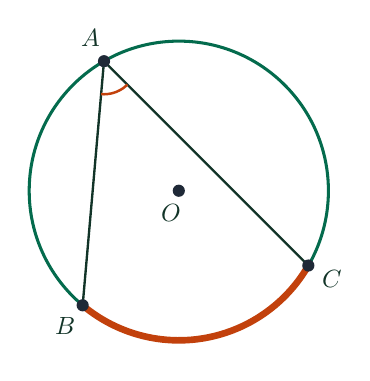
\begin{tikzpicture}
\draw[color={rgb,255:red,4;green,107;blue,77}, line width=1.1pt] (0,0) circle (1.900);
\draw[color={rgb,255:red,194;green,65;blue,12}, line width=2.4pt] (230.000:1.900) arc[start angle=230.000, end angle=330.000, radius=1.900cm];
\draw[ink, line width=0.85pt] (-0.950,1.645) -- (-1.221,-1.455);
\draw[ink, line width=0.85pt] (-0.950,1.645) -- (1.645,-0.950);
\draw[color={rgb,255:red,194;green,65;blue,12}, line width=0.9pt] (-0.987,1.227) -- (-0.968,1.226) -- (-0.950,1.225) -- (-0.932,1.226) -- (-0.913,1.227) -- (-0.895,1.229) -- (-0.877,1.232) -- (-0.859,1.235) -- (-0.841,1.240) -- (-0.824,1.245) -- (-0.806,1.251) -- (-0.789,1.257) -- (-0.773,1.265) -- (-0.756,1.273) -- (-0.740,1.282) -- (-0.724,1.291) -- (-0.709,1.301) -- (-0.694,1.312) -- (-0.680,1.324) -- (-0.666,1.336) -- (-0.653,1.348);
\fill[color={rgb,255:red,31;green,41;blue,55}] (-0.950,1.645) circle (2.2pt);
\fill[color={rgb,255:red,31;green,41;blue,55}] (-1.221,-1.455) circle (2.2pt);
\fill[color={rgb,255:red,31;green,41;blue,55}] (1.645,-0.950) circle (2.2pt);
\fill[color={rgb,255:red,31;green,41;blue,55}] (0.000,0.000) circle (2.2pt);
\node[font=\small, text=ink, inner sep=0.5pt] at (-1.120,1.940) {$A$};
\node[font=\small, text=ink, inner sep=0.5pt] at (-1.440,-1.716) {$B$};
\node[font=\small, text=ink, inner sep=0.5pt] at (1.940,-1.120) {$C$};
\node[font=\small, text=ink, inner sep=0.5pt] at (-0.103,-0.282) {$O$};
\end{tikzpicture}
\end{document}
